\chapter{Simulations}
\label{ch:simulations}

\section{Why simulations?}

Simulations are used to check if the data we see is what we expected.



\section{Monte Carlo extensive air shower simulation}

For the simulation of air showers there are several programs available,
most notably \corsika and AIRES. \corsika was chosen because it is still
being actively worked on, unlike AIRES which received its last update in
2006. \corsika also includes updated models based on recent LHC data.
Additionally, \corsika is also used by most other cosmic-ray
experiments.

\corsika version 74000 is used. \corsika provides the choice from many
models for various interactions. For high energy hadronic interactions;
DPMJET 2.55, EPOS LHC\cite{pierog2013}, NEXUS 3.97, QGSJET 01C,
QGSJETII-04\cite{ostapchenko2013}, SIBYLL 2.1, and VENUS 4.12 are
available. For hadrons with energies below \SI{80}{\giga\electronvolt}
GHEISHA 2002d\cite{fesefeldt1985}, FLUKA, or URQMD 1.3cr can be
selected. Electromagnetic interactions can be treated by EGS4\cite{egs4}
code or by NKG formulas.

QGSJETII, GHEISHA and EGS4 were chosen. One configuration of \corsika
was compiled and all showers were run using that executable.

The simulations are steered by an input file, many parameters can be set
here. The default options were used whenever applicable and trusting in
sensibly chosen defaults. The seeds for the random number generators
(first for the hadron shower, second for EGS4) are different for each
run. The seed values are (by us) also used as identifiers for the
simulations, so each combination of two seeds is unique in dataset of
simulations. Only one shower is simulated per run. Each run is for a
specific particle with a specified energy between
\SIrange{e12}{e18}{\electronvolt} in steps of $\log E = .5$.
The zenith angle is also set for each run and can be varied from
\SIrange{0}{60}{\degree} in steps of \SI{7.5}{\degree}. The azimuthal
angle is usually set to \SI{0}{\degree} (\hisparc coordinate system). 
The magnetic field values have been modified to values for Amsterdam [ref].

Energy cuts \SI{300}{\mega\electronvolt} for hadrons and muons, and
\SI{3}{\mega\electronvolt} for electrons and photons. Below these
energies the particles are quickly stopped/slowed by the atmosphere
decay [ref PDG]. The observation level for all runs is set to
\SI{10}{\meter} above sea level, which is relevant for the Science Park
where ground level is \SI{3.7}{\meter} below sea level, and the detector
are on the roofs of buildings.


\subsection{Stoomboot}

To run a significant number of simulations the local Nikhef
computer cluster 'Stoomboot' was utilized. This cluster used to have
around 300 CPUs available, but was expanded in February 2014 to 850
CPUs. Job queueing uses a fair-use policy to give each group at Nikhef
equal access to computation time.

Simulation time for each simulation is different because the number of
particles in a simulations will be different each run. Stoomboot has a
maximum job time of \SI{96}{\hour}. This allows for showers with primary
energies upto \SI{e17}{\electronvolt}, which take around 60 hours to
complete. A large sample of showers can easily be generated by
running many jobs simultaneously.

Since there are also showers of energies \SI{e17}{\electronvolt} we
want to have some simulations at higher energies. During the 2014
Christmas holidays 285 jobs at energies
\SIrange{e17.5}{e18}{\electronvolt}. These jobs sometimes took over
\SI{400}{\hour} to complete. This was a special run where the maximum
jobs times had to be explicitly set by the administrators. In total we
used \SI{50}{\year} of compute time to generate the simulation sample.

\todo{Determine compute time used on Stoomboot}

\begin{figure}
    \centering
    % \usepackage{tikz}
% \usetikzlibrary{arrows,external}
% \usepackage{pgfplots}
% \pgfplotsset{compat=1.3}
% \usepackage[detect-family]{siunitx}
% \usepackage[eulergreek]{sansmath}
% \sisetup{text-sf=\sansmath}
% \usepackage{relsize}
%
    \tikzsetnextfilename{externalized-shower_walltime}
\pgfkeysifdefined{/artist/width}
    {\pgfkeysgetvalue{/artist/width}{\defaultwidth}}
    {\def\defaultwidth{ .67\linewidth }}
%
%
\begin{sansmath}
\begin{tikzpicture}[
        font=\sffamily,
        every pin/.style={inner sep=2pt, font={\sffamily\smaller}},
        every label/.style={inner sep=2pt, font={\sffamily\smaller}},
        every pin edge/.style={<-, >=stealth', shorten <=2pt},
        pin distance=2.5ex,
    ]
    \begin{axis}[
            axis background/.style={  },
            xmode=log,
            ymode=normal,
            width=\defaultwidth,
            scale only axis,
            axis equal=false,
            %
            title={  },
            %
            xlabel={ Walltime [\si{\hour}] },
            ylabel={ Count },
            %
            xmin={  },
            xmax={  },
            ymin={ 0 },
            ymax={  },
            %
            xtick={  },
            ytick={  },
            xticklabel style={  },
            yticklabel style={  },
            %
            tick align=outside,
            max space between ticks=40,
            every tick/.style={},
            axis on top,
            point meta min={  },
            point meta max={  },
                colormap={coolwarm}{
                    rgb255(0cm)=( 59, 76,192);
                    rgb255(1cm)=( 98,130,234);
                    rgb255(2cm)=(141,176,254);
                    rgb255(3cm)=(184,208,249);
                    rgb255(4cm)=(221,221,221);
                    rgb255(5cm)=(245,196,173);
                    rgb255(6cm)=(244,154,123);
                    rgb255(7cm)=(222, 96, 77);
                    rgb255(8cm)=(180,  4, 38)},
        ]

        


    
    % Draw series plot
    \addplot[no markers,solid,const plot] coordinates {
            (0.0036416653952, 871)
            (0.0038629679752, 1619)
            (0.00409771902632, 988)
            (0.0043467358069, 160)
            (0.00461088523971, 21)
            (0.00489108693012, 2)
            (0.00518831636753, 27)
            (0.00550360832145, 170)
            (0.00583806044395, 1064)
            (0.00619283709095, 1180)
            (0.00656917337587, 1068)
            (0.00696837946945, 691)
            (0.00739184516101, 299)
            (0.00784104469682, 257)
            (0.00831754191251, 528)
            (0.00882299567741, 744)
            (0.00935916566966, 776)
            (0.00992791850238, 704)
            (0.010531234222, 415)
            (0.0111712132017, 153)
            (0.0118500834533, 61)
            (0.0125702083843, 524)
            (0.0133340950254, 519)
            (0.0141444027585, 21)
            (0.0150039525752, 13)
            (0.0159157368977, 7)
            (0.0168829299964, 1)
            (0.017908899041, 2)
            (0.0189972158226, 0)
            (0.0201516691889, 1)
            (0.0213762782342, 0)
            (0.0226753062916, 0)
            (0.0240532757753, 1)
            (0.025514983925, 39)
            (0.0270655195065, 296)
            (0.0287102805281, 619)
            (0.030454993033, 433)
            (0.0323057310335, 368)
            (0.0342689376575, 586)
            (0.0363514475794, 956)
            (0.0385605108136, 1262)
            (0.0409038179556, 1110)
            (0.0433895269549, 1034)
            (0.0460262915167, 922)
            (0.0488232912284, 940)
            (0.0517902635173, 1149)
            (0.0549375375503, 1157)
            (0.0582760701939, 701)
            (0.0618174841588, 198)
            (0.0655741084636, 114)
            (0.0695590213562, 174)
            (0.0737860958449, 578)
            (0.078270047995, 63)
            (0.0830264881613, 564)
            (0.0880719753339, 34)
            (0.0934240747862, 0)
            (0.0991014192263, 4)
            (0.105123773665, 11)
            (0.111512104224, 55)
            (0.11828865113, 45)
            (0.125477006138, 43)
            (0.133102194664, 19)
            (0.141190762912, 10)
            (0.149770870284, 5)
            (0.158872387421, 0)
            (0.168527000191, 1)
            (0.178768319997, 1)
            (0.189632000798, 2)
            (0.201155863228, 1)
            (0.213380026264, 0)
            (0.226347046901, 1)
            (0.240102068304, 2)
            (0.254692976972, 7)
            (0.270170569445, 12)
            (0.286588729152, 211)
            (0.304004613995, 1348)
            (0.32247885534, 894)
            (0.342075769098, 583)
            (0.36286357963, 1590)
            (0.384914657267, 2904)
            (0.408305770258, 2482)
            (0.433118352025, 1230)
            (0.459438784669, 1041)
            (0.487358699699, 1421)
            (0.516975297031, 1443)
            (0.548391683386, 1264)
            (0.581717231236, 833)
            (0.617067959579, 543)
            (0.654566937841, 497)
            (0.694344714327, 75)
            (0.736539770713, 76)
            (0.781299004152, 262)
            (0.82877823868, 12)
            (0.879142767697, 1)
            (0.93256792942, 1)
            (0.989239717299, 0)
            (1.04935542754, 2)
            (1.11312434594, 4)
            (1.18076847655, 30)
            (1.25252331448, 87)
            (1.32863866582, 48)
            (1.40937951725, 9)
            (1.4950269586, 0)
            (1.58587916143, 2)
            (1.68225241704, 0)
            (1.78448223766, 1)
            (1.89292452445, 2)
            (2.00795680653, 2)
            (2.12997955535, 1)
            (2.25941757884, 0)
            (2.39672150032, 0)
            (2.54236932735, 1)
            (2.69686811578, 2)
            (2.86075573509, 7)
            (3.03460274085, 9)
            (3.21901436107, 37)
            (3.41463260323, 572)
            (3.62213848937, 3599)
            (3.84225442695, 1759)
            (4.07574672386, 1899)
            (4.32342825622, 1248)
            (4.5861612983, 954)
            (4.86486052447, 1215)
            (5.16049619348, 2520)
            (5.47409752632, 2001)
            (5.80675628935, 1315)
            (6.15963059515, 1420)
            (6.53394893432, 659)
            (6.93101445238, 103)
            (7.35220948648, 146)
            (7.79900037787, 50)
            (8.27294257677, 0)
            (8.77568605749, 0)
            (9.30898106267, 1)
            (9.87468419648, 0)
            (10.4747648882, 1)
            (11.1113122486, 5)
            (11.7865423427, 6)
            (12.5028059053, 25)
            (13.2625965241, 69)
            (14.0685593213, 24)
            (14.9235001621, 4)
            (15.8303954229, 1)
            (16.7924023536, 1)
            (17.8128700688, 3)
            (18.8953512074, 3)
            (20.0436143009, 6)
            (21.2616568929, 3)
            (22.5537194563, 4)
            (23.9243001557, 0)
            (25.3781705074, 1)
            (26.9203919912, 3)
            (28.5563336705, 1)
            (30.2916908851, 3)
            (32.132505078, 11)
            (34.0851848286, 16)
            (36.156528163, 47)
            (38.3537462206, 462)
            (40.6844883592, 1274)
            (43.1568687849, 1089)
            (45.7794948008, 866)
            (48.5614967727, 228)
            (51.5125599151, 145)
            (54.6429580089, 114)
            (57.9635891691, 120)
            (61.4860137845, 209)
            (65.2224947644, 168)
            (69.1860402303, 23)
            (73.390448802, 17)
            (77.8503576362, 14)
            (82.5812933837, 6)
            (87.5997262441, 0)
            (92.9231273041, 0)
            (98.5700293619, 0)
            (104.560091446, 0)
            (110.914167258, 0)
            (117.654377769, 4)
            (124.804188233, 9)
            (132.388489879, 35)
            (140.433686565, 47)
            (148.967786705, 4)
            (158.020500767, 0)
            (167.623344718, 0)
            (177.809749736, 0)
            (188.615178598, 0)
            (200.07724914, 0)
            (212.23586522, 0)
            (225.133355639, 0)
            (238.814621499, 0)
            (253.327292529, 0)
            (268.721892893, 0)
            (285.052017094, 0)
            (302.374516547, 0)
            (320.749697508, 0)
            (340.241531021, 2)
            (360.917875624, 4)
            (382.850713591, 5)
            (406.116401532, 51)
            (430.795936219, 70)
            (456.975236565, 44)
            (484.745442741, 44)
    };


    \end{axis}
\end{tikzpicture}
\end{sansmath}
    \caption{\captitle{Walltime for \corsika simulations.}}
    \label{fig:simulations_shower_walltime}
\end{figure}


\subsection{No thinning}

\corsika provides a thinning mechanism to reduce the computation time.
Thinning looks at particles emerging from interactions and takes those
below a set fraction of the primary particle energy and drops all but
one of those. The particle that is kept is given a weight to represent
the dropped particles.

The thinning mechanism has not been enabled. Using Stoomboot enough
computational time (3 weeks) is available to run
\SI{e18}{\electronvolt} showers without thinning. Normally the long
queue on Stoomboot allows for jobs up to \SI{96}{\hour} walltime, for the
>\SI{e17}{\electronvolt} showers the jobs were extended by the
Stoomboot admins (Jeff) to \SI{2000}{\hour} to ensure the jobs had
enough time to finish.

[graph of run time vs shower size/zenith/energy]

For higher energies thinning might be required to keep run times
reasonable. However, thinned data provides different output, not one
particle for each particle on the ground, instead it stops following
some particles in the shower and assigns weights to those that remain.

Dethinning http://www.icrr.u-tokyo.ac.jp/~fukushim/WEB/pap/dethinning.pdf

Number of showers detected above \SI{e18}{\electronvolt} is minimal with \hisparc


\subsection{Simulations catalogue}

Using Stoomboot a collection of over \num{70000} simulated showers has
been created. This data is stored on the \hisparc data server (trave)
which has \SI{37}{\tera\byte} space. This space is shared with the raw
\hisparc data, \knmi lightning data, and some analysis files from
various \hisparc collaborators.

For easy use with the \sapphire framework the \corsika simulations are
converted from the binary/fortran data format to \hdf format. This is
done using a modified version of the the Python \corsika Reader by J.
Gonzalez from Auger [dead link]. During the conversion the values are
(when applicable) converted to the units and coordinate system used in
\hisparc [see appendix].

After the initial conversion further optimisation is performed by
sorting and indexing the 'x' coordinate column for the particles. In the
detector simulation particles are queried from the \corsika data file
using x and y coordinates. With the index it is very easy for the
software to know which part of the data it needs, since the data is
sorted (on disk) only a small part of the data needs to be read into
memory, if the data was not sorted more chunks of the file would need to
be read into memory. In some cases the sorting speeds up simulations by
a factor of 50.

Given the high abundance of protons as primary particles and iron with a
relative high abundance for heavier nuclei we have mostly focused on
those two particles for the simulations. However, some other primaries
have also been used. For protons (and iron??) all possible combinations
of energy and zenith have been simulated at least x times. More showers
are available at lower zenith angles and around
\SI{e15}{\electronvolt}. Larger showers take up much more disk
space and time to compute. In \ref{fig:simulations_proton_energy_zenith}
the number of simulations for each combination of parameters can be seen.
(at time of writing..)

\todo{Update plot with intermediate energies, and 'color bar'}

\begin{figure}
    \centering
    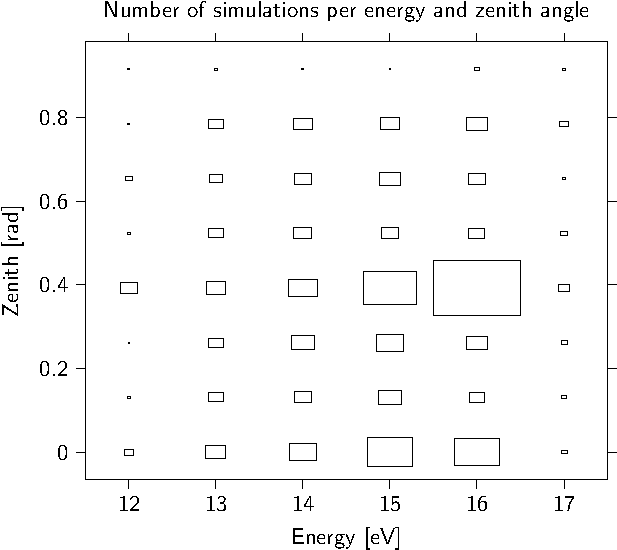
\includegraphics[width=0.7\linewidth]
        {plots/simulations/proton_energy_zenith}
    \caption{\captitle{Proton simulations overview.} The area of the
             rectangles indicate the number simulations with that energy
             and zenith combinations.}
    \label{fig:simulations_proton_energy_zenith}
\end{figure}


\subsubsection{Simulation overview}

In order to find a suitable \corsika simulation for detector simulations
an overview (\hdf) of all \corsika simulations is generated. The
overview contains the input parameters, the number of particles on
ground level, and the height of first interaction for each simulation.


\section{Detector simulation}

The detector and station responses and accuracies reported in [chapters
detector/station] are implemented in the simulations. These routines
provide the station response to air showers.

As input the \corsika showers can be used, but the simulation also
provides analytical functions that describe the particle densities as
function of the core distance (Ldf) and those that contain the time
structure of the shower front.

The same cluster objects (containing detector positions) that are used
in reconstructions are used as input for simulations.


\subsection{Simulation steps}

- Input cluster, \corsika data, max core distance, number of iterations, and an output file.

- For each iteration

- Generate shower parameters; core position, azimuth angle, and timestamp

- Instead of shifting and rotating the particles in the \corsika file
the cluster and detector positions are shifted.

- Then for each station each detector is simulated
- For each detector we check which particles pass through it, and then determine the detector response (total signal strength and time of first particle).
- Then it is determined if the station triggered or not.
- Then save events
- Save coincidence with links to events and shower paramters, also save
coincidence if there are no events.

%trigger efficiency
%simulations
%every step explained and understood
%trigger representateren


\section{Simulations on clusters}

We have some simple simulations for flat and curved shower fronts.
Does not include particle density.
Detector/trigger/response simulations. Do we understand what we see?


\section{Realistic simulation}

\todo{Simulation with fluxes and azimuth/zenith distributions.}

\todo{Acceptance; angle, energy and particles.}

See detector response, cluster response and calibration.


\section{Analysis}

\todo{Information about shower from simulations}

\begin{figure}
    \centering
    % \usepackage{tikz}
% \usetikzlibrary{arrows,external}
% \usepackage{pgfplots}
% \pgfplotsset{compat=1.3}
% \usepackage[detect-family]{siunitx}
% \usepackage[eulergreek]{sansmath}
% \sisetup{text-sf=\sansmath}
% \usepackage{relsize}
%
    \tikzsetnextfilename{externalized-shower_sizes}
\pgfkeysifdefined{/artist/width}
    {\pgfkeysgetvalue{/artist/width}{\defaultwidth}}
    {\def\defaultwidth{ .67\linewidth }}
%
%
\begin{sansmath}
\begin{tikzpicture}[
        font=\sffamily,
        every pin/.style={inner sep=2pt, font={\sffamily\smaller}},
        every label/.style={inner sep=2pt, font={\sffamily\smaller}},
        every pin edge/.style={<-, >=stealth', shorten <=2pt},
        pin distance=2.5ex,
    ]
    \begin{axis}[
            axis background/.style={  },
            xmode=normal,
            ymode=log,
            width=\defaultwidth,
            scale only axis,
            axis equal=false,
            %
            title={  },
            %
            xlabel={ Zenith [\si{\radian}] },
            ylabel={ Shower size (leptons) },
            %
            xmin={  },
            xmax={  },
            ymin={  },
            ymax={  },
            %
            xtick={  },
            ytick={  },
            xticklabel style={  },
            yticklabel style={  },
            %
            tick align=outside,
            max space between ticks=40,
            every tick/.style={},
            axis on top,
            point meta min={  },
            point meta max={  },
                colormap={coolwarm}{
                    rgb255(0cm)=( 59, 76,192);
                    rgb255(1cm)=( 98,130,234);
                    rgb255(2cm)=(141,176,254);
                    rgb255(3cm)=(184,208,249);
                    rgb255(4cm)=(221,221,221);
                    rgb255(5cm)=(245,196,173);
                    rgb255(6cm)=(244,154,123);
                    rgb255(7cm)=(222, 96, 77);
                    rgb255(8cm)=(180,  4, 38)},
        ]

        


    \addplot[draw=none, fill=lightgray,semitransparent] coordinates {
            (0.0, 11382.32)
            (0.1309, 11341.72)
            (0.261799, 12438.0)
            (0.392699, 8049.92)
            (0.523599, 7857.68)
            (0.654498, 4526.32)
            (0.785398, 2570.32)
            (0.916298, 1866.2)
            (1.0472, 1255.32)
            (1.0472, 2253.52)
            (0.916298, 2965.04)
            (0.785398, 5894.72)
            (0.654498, 10405.0)
            (0.523599, 19943.2)
            (0.392699, 24771.12)
            (0.261799, 24461.44)
            (0.1309, 37076.92)
            (0.0, 47313.76)
            } -- cycle;

    \addplot[draw=none, fill=lightgray,semitransparent] coordinates {
            (0.0, 631.2)
            (0.1309, 657.56)
            (0.261799, 630.88)
            (0.392699, 324.8)
            (0.523599, 476.44)
            (0.654498, 407.76)
            (0.785398, 309.36)
            (0.916298, 273.8)
            (1.0472, 163.88)
            (1.0472, 319.0)
            (0.916298, 409.44)
            (0.785398, 351.36)
            (0.654498, 595.0)
            (0.523599, 1162.96)
            (0.392699, 1067.2)
            (0.261799, 1698.84)
            (0.1309, 1989.32)
            (0.0, 1668.52)
            } -- cycle;

    \addplot[draw=none, fill=lightgray,semitransparent] coordinates {
            (0.261799, 37247828.0)
            (0.392699, 34000685.76)
            (0.523599, 22196393.76)
            (0.654498, 12001765.76)
            (0.785398, 5201100.2)
            (0.916298, 1779225.68)
            (1.0472, 906333.52)
            (1.0472, 1328089.76)
            (0.916298, 3738917.72)
            (0.785398, 8480915.2)
            (0.654498, 20569885.92)
            (0.523599, 29420888.16)
            (0.392699, 43290873.6)
            (0.261799, 40378553.44)
            } -- cycle;

    \addplot[draw=none, fill=lightgray,semitransparent] coordinates {
            (0.0, 199062.44)
            (0.1309, 184078.96)
            (0.261799, 186163.28)
            (0.392699, 123920.2)
            (0.523599, 88336.24)
            (0.654498, 64867.0)
            (0.785398, 29158.6)
            (0.916298, 17920.52)
            (1.0472, 14137.32)
            (1.0472, 17985.36)
            (0.916298, 35205.68)
            (0.785398, 60415.96)
            (0.654498, 253588.08)
            (0.523599, 208427.92)
            (0.392699, 404007.56)
            (0.261799, 327410.48)
            (0.1309, 460465.32)
            (0.0, 510995.56)
            } -- cycle;

    \addplot[draw=none, fill=lightgray,semitransparent] coordinates {
            (0.0, 16.0)
            (0.1309, 16.0)
            (0.261799, 16.0)
            (0.392699, 14.0)
            (0.523599, 14.0)
            (0.654498, 13.0)
            (0.785398, 11.0)
            (0.916298, 8.84)
            (0.916298, 19.16)
            (0.785398, 23.16)
            (0.654498, 27.0)
            (0.523599, 31.0)
            (0.392699, 35.0)
            (0.261799, 38.16)
            (0.1309, 44.16)
            (0.0, 48.0)
            } -- cycle;

    \addplot[draw=none, fill=lightgray,semitransparent] coordinates {
            (0.0, 169.0)
            (0.1309, 182.0)
            (0.261799, 146.24)
            (0.392699, 132.0)
            (0.523599, 118.0)
            (0.654498, 101.24)
            (0.785398, 83.0)
            (0.916298, 70.84)
            (1.0472, 66.68)
            (1.0472, 116.32)
            (0.916298, 135.48)
            (0.785398, 167.76)
            (0.654498, 226.52)
            (0.523599, 341.76)
            (0.392699, 414.52)
            (0.261799, 518.8)
            (0.1309, 639.16)
            (0.0, 609.76)
            } -- cycle;

    \addplot[draw=none, fill=lightgray,semitransparent] coordinates {
            (0.0, 2853.4)
            (0.1309, 2701.16)
            (0.261799, 2350.12)
            (0.392699, 1798.44)
            (0.523599, 1451.12)
            (0.654498, 1028.0)
            (0.785398, 807.72)
            (0.916298, 662.04)
            (1.0472, 536.68)
            (1.0472, 788.16)
            (0.916298, 1092.96)
            (0.785398, 1698.84)
            (0.654498, 2903.76)
            (0.523599, 5344.28)
            (0.392699, 6860.12)
            (0.261799, 9083.84)
            (0.1309, 9761.56)
            (0.0, 10130.64)
            } -- cycle;

    \addplot[draw=none, fill=lightgray,semitransparent] coordinates {
            (0.0, 55136.12)
            (0.1309, 51547.4)
            (0.261799, 44947.24)
            (0.392699, 33723.4)
            (0.523599, 22061.84)
            (0.654498, 13799.28)
            (0.785398, 8706.2)
            (0.916298, 5919.8)
            (1.0472, 4005.12)
            (1.0472, 6357.6)
            (0.916298, 10099.68)
            (0.785398, 20933.92)
            (0.654498, 38118.72)
            (0.523599, 68579.56)
            (0.392699, 101335.0)
            (0.261799, 133711.68)
            (0.1309, 151807.64)
            (0.0, 166450.84)
            } -- cycle;

    \addplot[draw=none, fill=lightgray,semitransparent] coordinates {
            (0.0, 933444.84)
            (0.1309, 890634.36)
            (0.261799, 755564.88)
            (0.392699, 569171.24)
            (0.523599, 369110.8)
            (0.654498, 200854.24)
            (0.785398, 101316.6)
            (0.916298, 56003.6)
            (1.0472, 34741.2)
            (1.0472, 51160.28)
            (0.916298, 97492.36)
            (0.785398, 219722.8)
            (0.654498, 537116.16)
            (0.523599, 930104.2)
            (0.392699, 1412316.92)
            (0.261799, 1861482.28)
            (0.1309, 1999034.92)
            (0.0, 2168503.84)
            } -- cycle;

    \addplot[draw=none, fill=lightgray,semitransparent] coordinates {
            (0.0, 14051766.36)
            (0.1309, 13798365.0)
            (0.261799, 11654958.8)
            (0.392699, 8740413.16)
            (0.523599, 5463975.44)
            (0.654498, 2883176.16)
            (0.785398, 1286342.76)
            (0.916298, 575788.4)
            (1.0472, 327520.4)
            (1.0472, 447841.64)
            (0.916298, 973584.76)
            (0.785398, 2886783.12)
            (0.654498, 7839064.24)
            (0.523599, 12967109.12)
            (0.392699, 17937112.08)
            (0.261799, 25781858.0)
            (0.1309, 26230808.0)
            (0.0, 28442164.8)
            } -- cycle;

    \addplot[draw=none, fill=lightgray,semitransparent] coordinates {
            (0.654498, 36715305.92)
            (0.785398, 16066389.36)
            (0.916298, 6209193.56)
            (1.0472, 3079834.76)
            (1.0472, 3563681.28)
            (0.916298, 10707477.12)
            (0.785398, 23453379.2)
            (0.654498, 40468008.96)
            } -- cycle;

    \addplot[draw=none, fill=lightgray,semitransparent] coordinates {
            (0.0, 3432960.72)
            (0.1309, 3390485.4)
            (0.261799, 3053419.24)
            (0.392699, 2867473.28)
            (0.523599, 1442700.56)
            (0.654498, 776463.32)
            (0.785398, 343483.36)
            (0.916298, 176362.04)
            (1.0472, 98726.44)
            (1.0472, 152729.32)
            (0.916298, 292981.96)
            (0.785398, 752531.56)
            (0.654498, 2502825.92)
            (0.523599, 3601883.96)
            (0.392699, 4744789.04)
            (0.261799, 7158101.84)
            (0.1309, 7388482.2)
            (0.0, 9846644.96)
            } -- cycle;

    
    % Draw series plot
    \addplot[mark=*,mark options=white,only marks] coordinates {
            (0.0, 4.37281e+06)
            (0.1309, 5.4088e+06)
            (0.261799, 4.89299e+06)
            (0.392699, 3.38686e+06)
            (0.523599, 1.84289e+06)
            (0.654498, 1.23085e+06)
            (0.785398, 582579.0)
            (0.916298, 199512.0)
            (1.0472, 130062.0)
    };

    
    % Draw series plot
    \addplot[mark=*,mark options=white,only marks] coordinates {
            (0.654498, 4.01265e+07)
            (0.785398, 2.00544e+07)
            (0.916298, 7.93248e+06)
            (1.0472, 3.25808e+06)
    };

    
    % Draw series plot
    \addplot[mark=*,mark options=white,only marks] coordinates {
            (0.0, 1.87288e+07)
            (0.1309, 1.73035e+07)
            (0.261799, 1.59842e+07)
            (0.392699, 1.18518e+07)
            (0.523599, 7.70421e+06)
            (0.654498, 4.46561e+06)
            (0.785398, 1.73332e+06)
            (0.916298, 713648.0)
            (1.0472, 393638.0)
    };

    
    % Draw series plot
    \addplot[mark=*,mark options=white,only marks] coordinates {
            (0.0, 1.33579e+06)
            (0.1309, 1.27176e+06)
            (0.261799, 1.09588e+06)
            (0.392699, 834848.0)
            (0.523599, 549684.0)
            (0.654498, 305770.0)
            (0.785398, 137276.0)
            (0.916298, 69467.0)
            (1.0472, 43057.0)
    };

    
    % Draw series plot
    \addplot[mark=*,mark options=white,only marks] coordinates {
            (0.0, 88484.0)
            (0.1309, 81400.0)
            (0.261799, 72721.5)
            (0.392699, 54856.0)
            (0.523599, 36047.5)
            (0.654498, 21661.0)
            (0.785398, 11874.0)
            (0.916298, 7790.0)
            (1.0472, 5226.5)
    };

    
    % Draw series plot
    \addplot[mark=*,mark options=white,only marks] coordinates {
            (0.0, 5043.5)
            (0.1309, 5117.5)
            (0.261799, 4144.0)
            (0.392699, 3174.5)
            (0.523599, 2407.5)
            (0.654498, 1555.5)
            (0.785398, 1110.0)
            (0.916298, 863.0)
            (1.0472, 658.5)
    };

    
    % Draw series plot
    \addplot[mark=*,mark options=white,only marks] coordinates {
            (0.0, 287.0)
            (0.1309, 299.0)
            (0.261799, 248.0)
            (0.392699, 209.0)
            (0.523599, 188.0)
            (0.654498, 149.5)
            (0.785398, 120.0)
            (0.916298, 97.0)
            (1.0472, 82.5)
    };

    
    % Draw series plot
    \addplot[mark=*,mark options=white,only marks] coordinates {
            (0.0, 28.5)
            (0.1309, 26.0)
            (0.261799, 24.0)
            (0.392699, 22.0)
            (0.523599, 21.0)
            (0.654498, 19.0)
            (0.785398, 17.0)
            (0.916298, 13.0)
    };

    
    % Draw series plot
    \addplot[mark=*,mark options=white,only marks] coordinates {
            (0.0, 383208.0)
            (0.1309, 312196.0)
            (0.261799, 268031.0)
            (0.392699, 210422.0)
            (0.523599, 135921.0)
            (0.654498, 118724.0)
            (0.785398, 42832.5)
            (0.916298, 23830.0)
            (1.0472, 15279.0)
    };

    
    % Draw series plot
    \addplot[mark=*,mark options=white,only marks] coordinates {
            (0.261799, 3.95884e+07)
            (0.392699, 3.87502e+07)
            (0.523599, 2.62175e+07)
            (0.654498, 1.5439e+07)
            (0.785398, 6.37078e+06)
            (0.916298, 2.50866e+06)
            (1.0472, 1.1277e+06)
    };

    
    % Draw series plot
    \addplot[mark=*,mark options=white,only marks] coordinates {
            (0.0, 1174.5)
            (0.1309, 1347.5)
            (0.261799, 1035.5)
            (0.392699, 658.0)
            (0.523599, 544.5)
            (0.654498, 520.5)
            (0.785398, 329.5)
            (0.916298, 355.5)
            (1.0472, 234.5)
    };

    
    % Draw series plot
    \addplot[mark=*,mark options=white,only marks] coordinates {
            (0.0, 14349.0)
            (0.1309, 17555.0)
            (0.261799, 19999.5)
            (0.392699, 12572.0)
            (0.523599, 11831.5)
            (0.654498, 6237.0)
            (0.785398, 3536.0)
            (0.916298, 2383.5)
            (1.0472, 1750.0)
    };

    
    % Draw series plot
    \addplot[mark=o,solid] coordinates {
            (0.0, 14349.0)
            (0.1309, 17555.0)
            (0.261799, 19999.5)
            (0.392699, 12572.0)
            (0.523599, 11831.5)
            (0.654498, 6237.0)
            (0.785398, 3536.0)
            (0.916298, 2383.5)
            (1.0472, 1750.0)
    };

    
    % Draw series plot
    \addplot[mark=o,solid] coordinates {
            (0.0, 1174.5)
            (0.1309, 1347.5)
            (0.261799, 1035.5)
            (0.392699, 658.0)
            (0.523599, 544.5)
            (0.654498, 520.5)
            (0.785398, 329.5)
            (0.916298, 355.5)
            (1.0472, 234.5)
    };

    
    % Draw series plot
    \addplot[mark=o,solid] coordinates {
            (0.261799, 3.95884e+07)
            (0.392699, 3.87502e+07)
            (0.523599, 2.62175e+07)
            (0.654498, 1.5439e+07)
            (0.785398, 6.37078e+06)
            (0.916298, 2.50866e+06)
            (1.0472, 1.1277e+06)
    };

    
    % Draw series plot
    \addplot[mark=o,solid] coordinates {
            (0.0, 383208.0)
            (0.1309, 312196.0)
            (0.261799, 268031.0)
            (0.392699, 210422.0)
            (0.523599, 135921.0)
            (0.654498, 118724.0)
            (0.785398, 42832.5)
            (0.916298, 23830.0)
            (1.0472, 15279.0)
    };

    
    % Draw series plot
    \addplot[mark=o,solid] coordinates {
            (0.0, 28.5)
            (0.1309, 26.0)
            (0.261799, 24.0)
            (0.392699, 22.0)
            (0.523599, 21.0)
            (0.654498, 19.0)
            (0.785398, 17.0)
            (0.916298, 13.0)
    };

    
    % Draw series plot
    \addplot[mark=o,solid] coordinates {
            (0.0, 287.0)
            (0.1309, 299.0)
            (0.261799, 248.0)
            (0.392699, 209.0)
            (0.523599, 188.0)
            (0.654498, 149.5)
            (0.785398, 120.0)
            (0.916298, 97.0)
            (1.0472, 82.5)
    };

    
    % Draw series plot
    \addplot[mark=o,solid] coordinates {
            (0.0, 5043.5)
            (0.1309, 5117.5)
            (0.261799, 4144.0)
            (0.392699, 3174.5)
            (0.523599, 2407.5)
            (0.654498, 1555.5)
            (0.785398, 1110.0)
            (0.916298, 863.0)
            (1.0472, 658.5)
    };

    
    % Draw series plot
    \addplot[mark=o,solid] coordinates {
            (0.0, 88484.0)
            (0.1309, 81400.0)
            (0.261799, 72721.5)
            (0.392699, 54856.0)
            (0.523599, 36047.5)
            (0.654498, 21661.0)
            (0.785398, 11874.0)
            (0.916298, 7790.0)
            (1.0472, 5226.5)
    };

    
    % Draw series plot
    \addplot[mark=o,solid] coordinates {
            (0.0, 1.33579e+06)
            (0.1309, 1.27176e+06)
            (0.261799, 1.09588e+06)
            (0.392699, 834848.0)
            (0.523599, 549684.0)
            (0.654498, 305770.0)
            (0.785398, 137276.0)
            (0.916298, 69467.0)
            (1.0472, 43057.0)
    };

    
    % Draw series plot
    \addplot[mark=o,solid] coordinates {
            (0.0, 1.87288e+07)
            (0.1309, 1.73035e+07)
            (0.261799, 1.59842e+07)
            (0.392699, 1.18518e+07)
            (0.523599, 7.70421e+06)
            (0.654498, 4.46561e+06)
            (0.785398, 1.73332e+06)
            (0.916298, 713648.0)
            (1.0472, 393638.0)
    };

    
    % Draw series plot
    \addplot[mark=o,solid] coordinates {
            (0.654498, 4.01265e+07)
            (0.785398, 2.00544e+07)
            (0.916298, 7.93248e+06)
            (1.0472, 3.25808e+06)
    };

    
    % Draw series plot
    \addplot[mark=o,solid] coordinates {
            (0.0, 4.37281e+06)
            (0.1309, 5.4088e+06)
            (0.261799, 4.89299e+06)
            (0.392699, 3.38686e+06)
            (0.523599, 1.84289e+06)
            (0.654498, 1.23085e+06)
            (0.785398, 582579.0)
            (0.916298, 199512.0)
            (1.0472, 130062.0)
    };

    \node[coordinate,
          label={ []left:{ 14.5 }}]
        at (axis cs:0.0, 14349.0) {};

    \node[coordinate,
          label={ []left:{ 13.5 }}]
        at (axis cs:0.0, 1174.5) {};

    \node[coordinate,
          label={ []left:{ 17.5 }}]
        at (axis cs:0.261799, 3.95884e+07) {};

    \node[coordinate,
          label={ []left:{ 15.5 }}]
        at (axis cs:0.0, 383208.0) {};

    \node[coordinate,
          label={ []left:{ 12.0 }}]
        at (axis cs:0.0, 28.5) {};

    \node[coordinate,
          label={ []left:{ 13.0 }}]
        at (axis cs:0.0, 287.0) {};

    \node[coordinate,
          label={ []left:{ 14.0 }}]
        at (axis cs:0.0, 5043.5) {};

    \node[coordinate,
          label={ []left:{ 15.0 }}]
        at (axis cs:0.0, 88484.0) {};

    \node[coordinate,
          label={ []left:{ 16.0 }}]
        at (axis cs:0.0, 1.33579e+06) {};

    \node[coordinate,
          label={ []left:{ 17.0 }}]
        at (axis cs:0.0, 1.87288e+07) {};

    \node[coordinate,
          label={ []left:{ 18.0 }}]
        at (axis cs:0.654498, 4.01265e+07) {};

    \node[coordinate,
          label={ []left:{ 16.5 }}]
        at (axis cs:0.0, 4.37281e+06) {};


    \end{axis}
\end{tikzpicture}
\end{sansmath}
    \caption{\captitle{Shower size versus zenith angle and primary energy.}
             Each line indicates the median shower size for a specific
             energy as a function of zenith angle. The gray area
             indicates the 16th and 84th percentile.}
    \label{fig:simulations_shower_sizes}
\end{figure}



Timing information, front shape, timing distribution, particle arrival times..
Air pressure dependence.

Particle density, effect of inclination..
